\chapter{اجزا و تکنولوژی‌ها}
%\thispagestyle{empty}

\section{مقدمه}
در این قسمت اجزا، قطعات و تکنولوژی‌های سخت‌افزای و نرم‌افزاری مورد استفاده در پروژه معرفی خواهند شد.

\section{رزبری‌پای مدل \lr{3A}}
امروزه با پیشرفت روزافزون تکنولوژی و ظهور پردازنده‌های کم‌مصرف آرم\LTRfootnote{\lr{ARM}}، حجم و وزن کامپیوترها هرروز کوچک‌تر و در عوض سرعت و قدرت آن‌ها افزایش می‌یابد. بردهای رزبری‌پای\cite{Raspberry} \LTRfootnote{\lr{ًRaspberry PI}} از جمله کوچک‌ترین و پرقدرت‌ترین بردهای کامپیوتری هستند که علاوه بر ابعاد کوچک و وزن کم، از سرعت و دقت بالایی برخوردارند. بردهای رزبری‌پای توسط بنیاد خیریه رزبری \LTRfootnote{\lr{ًRaspberry Foundation}} و با هدف گسترش و توسعه علوم رایانه برای دانش‌آموزان ساخته شده است، تا نسل آینده بهتر بتواند روش عملکرد رایانه‌ها را درک کند. این دستگاه کوچک با توانایی‌های بسیار بالا برای تمام سنین و علاقه‌مندان به مباحث برنامه‌نویسی و اینترنت‌اشیاء\LTRfootnote{\lr{Internet of Things}} کاربرد دارد. برد رزبری‌پای 3 دارای یک درگاه\LTRfootnote{\lr{Port}} استاندارد رابط چندرسانه‌ای وضوح بالا\LTRfootnote{\lr{High-Definition Multimedia Interface (HDMI)}} است که این برد را قادر می‌سازد به انواع تلویزیون‌ها و نمایشگرها متصل شود. همچنین این بورد برخلاف نسل‌های قبلی خود، دارای قابلیت اتصال به اینترنت بی‌سیم\LTRfootnote{\lr{Wifi}} و بلوتوث\LTRfootnote{\lr{Bluethooth}} داخلی است که در کنار یک درگاه شبکه اترنت\LTRfootnote{\lr{Ethernet}} در قسمت شبکه و اتصال به اینترنت و سایر شبکه‌ها چیزی کم ندارد. رزبری‌پای 3 در قسمت پردازنده مرکزی از چیپ چهار هسته‌ای \lr{Cortex-A53 BCM2837} شرکت برادکام\LTRfootnote{\lr{Broadcom Corporation}} استفاده می‌کند که بر اساس گفته بنیاد رزبری، تا 60 درصد سریع‌تر از نسل پیشین، یعنی رزبری‌پای 2 است. انطباق‌دهنده\LTRfootnote{\lr{Adaptor}} مورد نیاز برای این برد باید دارای ولتاژ ۵ ولت و جریان ۲ آمپر باشد که می‌توان از درگاه گذرگاه سریال سراسری \LTRfootnote{\lr{Universal Serial Bus (USB)}} برد رزبری‌پای نیز استفاده کرد ولی توصیه می‌شود تا با انطباق‌دهنده مخصوص راه‌اندازی گردد. این پردازنده قادر است در هر هسته با فرکانس 1.2 گیگاهرتز فعالیت کند. همچنین این برد در قسمت گرافیک و پردازنده گرافیکی رزبری‌پای پیشرفت چشمگیری داشته و با یک 
پردازنده‌ی گرافیکی 400 مگاهرتز از نوع \lr{Dual Core VideoCore IV GPU} همراه شده است. این پردازنده گرافیکی دوهسته‌ای اگرچه نمی‌تواند ویدئوها و بازی‌هایی با کیفیت \lr{4K} را پشتیبانی کند، ولی با این‌حال از پس اکثر کاربردهای روزمره بر می‌آید. حافظه داخلی رزبری‌پای 3، یک گیگابایت است که برای سیستم‌عامل‌های کم‌حجم مانند رزبرین\LTRfootnote{\lr{Raspbian}} و برخی نسخه‌های لینوکس و اندروید مناسب است. 
و اما تفاوت اصلی کامپیوترهای تک‌بردی مانند رزبری‌پای با سایر کامپیوترها، وجود تعداد نسبتاً زیادی درگاه ورودی و خروجی عام منظوره\LTRfootnote{\lr{General Purpose Input/Output (GPIO)}} است. این درگاه‌ها که تعداد آن در رزبری‌پای 40 عدد است، کاربردهای بسیار زیادی در اینترنت اشیاء و اتوماسیون صنعتی دارند. این درگاه توانایی اتصال رزبری‌پای را به سایر دستگاه‌ها و سنسورهای الکترونیکی و تعامل با آن‌ها را فراهم می‌کنند. اجزای رزبری‌پای استفاده شده در این پروژه در تصویر \ref{raspberry} نمایش داده شده است.

\begin{figure}[t!]
    \centering
    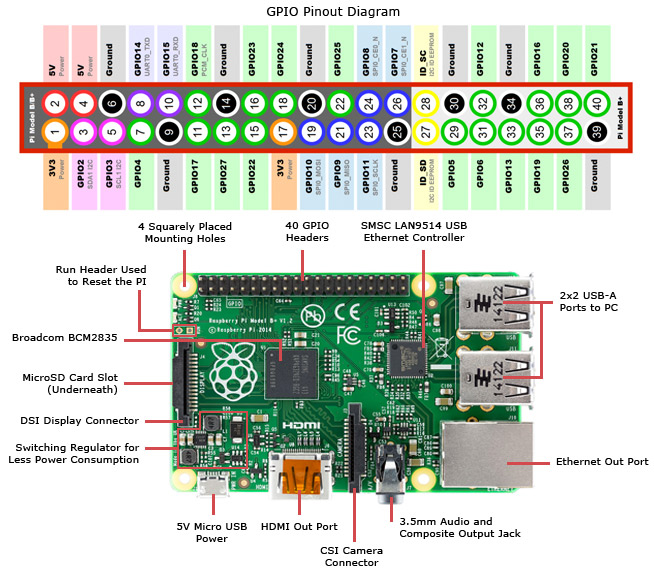
\includegraphics[scale=0.60]{figures/raspberry.jpg}
    \caption{اجزای رزبری‌پای مدل 3\lr{A}}
    \label{raspberry}
\end{figure}

\section{نمایشگر لمسی \lr{3.5} اینچی وِیوشِر}
این نمایشگر لمسی ساخت شرکت وِیوشِر\LTRfootnote{\lr{Waveshare}} بوده و دارای رزولوشن  {\lr{320x480} است. این نمایشگر را می‌توان برای انواع بوردهای رزبری‌پای مورد استفاده قرار داد. درایورهای این نمایشگر به صورت آماده بوده و به صورت مستقیم با  سیستم‌عامل رزبین هماهنگ است. اندازه‌ی این نمایشگر کاملاً با انواع بردهای رزبری‌پای مطابقت دارد و به راحتی بر روی آن قرار می‌گیرد. بر روی این نمایشگر می‌توان فیلم‌ها و عکس‌هایی با قالب‌\LTRfootnote{\lr{Format}} های مختلف و با کیفیتی بالا نمایش داد. این نمایشگر از نرم‌افزار صفحه‌کلید نیز پشتیبانی می‌کند که در این حالت نیازی به صفحه‌کلید خارجی نیست. صفحه لمسی این نمایشگر از نوع مقاومتی است. این نمایشگر در تصویر \ref{lcd} نشان داده شده است.

\begin{figure}[t!]
    \centering
    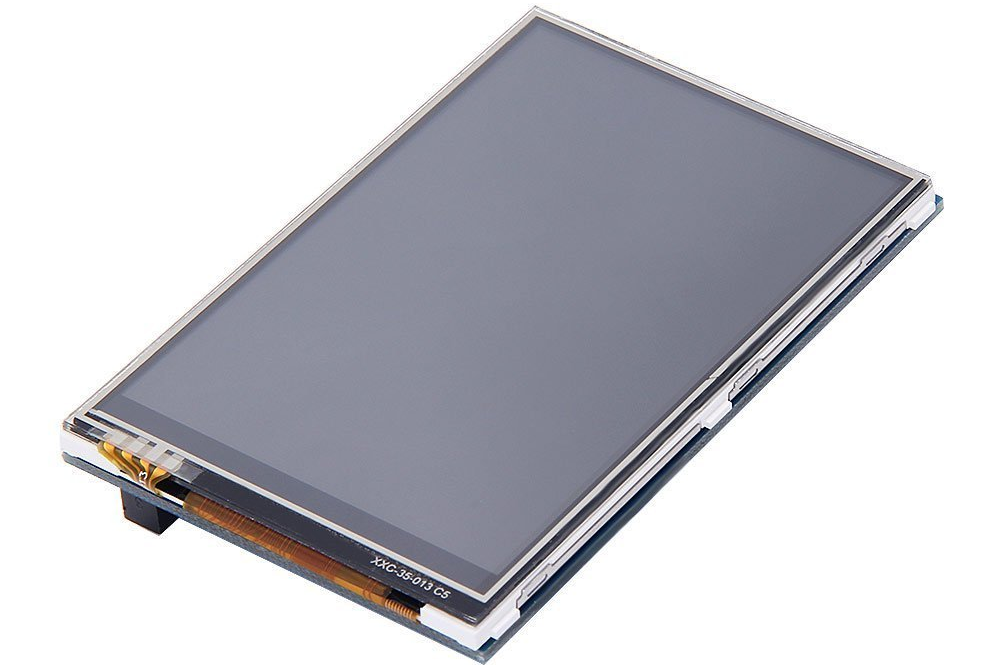
\includegraphics[scale=0.30]{figures/lcd.png}
    \caption{نمایشگر لمسی 3.5 اینچی}
    \label{lcd}
\end{figure}
\clearpage
برخی دیگر از ویژگی‌های این نمایشگر:

\begin{itemize}
	\item  یک جایگزین مناسب برای مانیتورهایی با رابط چندرسانه‌ای وضوح بالا
	\item پشتیبانی به‌وسیله درایورهای مورد نیاز
	\item پشتیبانی از سیستم‌عامل رزبین
	\item پشتیبانی از تمام نسخه‌های رزبری‌پای
	\item عکس‌برداری لمسی (در ۱۷ حالت دوربین)
	\item کیفیت بالای ساخت با روکش طلایی
	\item نمایشگر از جنس ترانزیستور فیلم نازک \LTRfootnote{\lr{TFT LCD}}
	\item رابط محیطی سریال \LTRfootnote{\lr{Serial Peripheral Interface (SPI)}}
	\item درایور لمسی \lr{XPT2046}
	\item پشتیبانی از ۶۵۵۳۶ رنگ مختلف
	\item نور پس‌زمینه از نوع دیود‌های ساطع‌کننده نور \LTRfootnote{\lr{Light-Emitting Diode (LED)}}
\end{itemize}


\section{سیستم‌عامل رزبین}
سیستم‌عامل نصب شده بر روی بورد رزبری‌پای، رزبین نام دارد. رزبین یک سیستم‌عامل رایانه‌ای مبتنی بر دبین\LTRfootnote{\lr{Debian}} برای رزبری‌پای است. نسخه‌های مختلفی از رزبین شامل \lr{Raspbian Buster} و \lr{Raspbian Stretch} وجود دارد.
این سیستم‌عامل را بنیاد رزبری از سال 2015 به طور رسمی به‌عنوان سیستم‌عامل اصلی برای خانواده رایانه‌های رزبری‌پای ارائه داده است. رزبین توسط مایک تامپسون\LTRfootnote{\lr{Mike Thompson}} و پیتر گرین\LTRfootnote{\lr{Peter Green}} به عنوان یک پروژه مستقل ایجاد شد. نسخه اولیه این سیستم‌عامل در ژوئن 2012 به پایان رسید. این سیستم‌عامل هنوز در حال توسعه است. رزبین برای پردازنده های آرم با توان پردازشی کم، بهینه شده است. رزبین در آخرین نسخه ارائه شده، از پیکسل\LTRfootnote{\lr{Pi Improved X-Window Environment, Lightweight(PIXEL)}} به عنوان محیط رومیزی\LTRfootnote{\lr{Desktop Enviorment}} خود استفاده می‌کند.

\section{چهارچوب نرم‌افزاری جنگو}
یک چهارچوب نرم‌افزاری\LTRfootnote{\lr{Software Framework}} سطح بالا، بسیاری از موارد برنامه نویسی را بصورت خودکار فراهم کرده و در اختیار برنامه نویس قرار می‌دهد . همچنین روش‌هایی میانبر و واسط برای اجرای اعمال مختلف را دارا است. این ویژگی باعث می‌شود برنامه‌نویس برای پیاده‌سازی بخش‌های مختلف کمتر کد بزند.
جنگو\cite{Django}\LTRfootnote{\lr{Django}}  یک چارچوب نرم‌افزاری آزاد و متن‌باز\LTRfootnote{\lr{Open Source}} مبتنی بر پایتون\LTRfootnote{\lr{Python}} است که امکان طراحی و ایجاد بسیار سریع و آسان برنامه‌های تحت وب را فراهم می‌کند. جنگو از الگوی معماری \lr{MTV}\LTRfootnote{\lr{Model Template View}} پیروی می‌کند. این مؤسسه توسط بنیاد نرم افزاری مستقل جنگو\LTRfootnote{\lr{Django Software Independent Foundation}} تأسیس شده و نگهداری می‌شود.
هدف اصلی جنگو، سهولت در ایجاد وب‌سایت‌های پیچیده و با محوریت پایگاه‌داده است. این چارچوب بر ویژگی‌هایی از جمله استفاده مجدد\LTRfootnote{\lr{Reusability}} و تعداد خط کد کم\LTRfootnote{\lr{Less Code}}، وابستگی کم\LTRfootnote{\lr{Low Coupling}}، توسعه سریع\LTRfootnote{\lr{Rapid Development}} و اصل تکرار خود\LTRfootnote{\lr{Don't repeat yourself (DRY)}} تأکید دارد.
در این پروژه برای پیاده‌سازی ساختار کلی \lr{Back-end} و همچنین رابط کاربری مدیریت از جنگو استفاده شده است.

\subsection{مزیت‌های جنگو}
در ادامه ویژگی‌های این چهارچوب قدرتمند توضیح داده خواهد شد.
\subsubsection{امکان جداسازی محتوا از ظاهر نمایشی}
در اکثر زبان‌های برنامه‌نویسی، کدهای زبان نشانه‌گذاری ابرمتنی با کدها و محتوای سایت آمیخته می‌گردند، که باعث ایجاد مشکلات هنگام تغییرات آتی و نگهداری می‌گردد . با استفاده از این روش ظاهر نمایشی سایت، بصورت جداگانه در فایلی خاص ذخیره می‌گردد . اکنون با اعمال تغییر در هر نوع محتوا، نیازی به ویرایش دیگری نیست و این دو موجودیت مستقل می‌باشند.

\subsubsection{لایه‌بندی}
در حالت معمول هر برنامه نوشته شده با جنگو دارای ۳ لایه مهم است. بخش نمایشی\LTRfootnote{\lr{Template}}، محتوا و یا کدهای کنترلی\LTRfootnote{\lr{View}} و بخش ذخیره دائمی اطلاعات\LTRfootnote{\lr{Model}}. البته با توجه به نوع برنامه و نیاز‌های برنامه‌نویس می‌توان این لایه‌ها را ادغام کرده یا نادیده گرفت. نحوه ارتباط این لایه‌ها در تصویر\ref{mtv} نشان داده شده است.
 
\begin{figure}[t!]
    \centering
    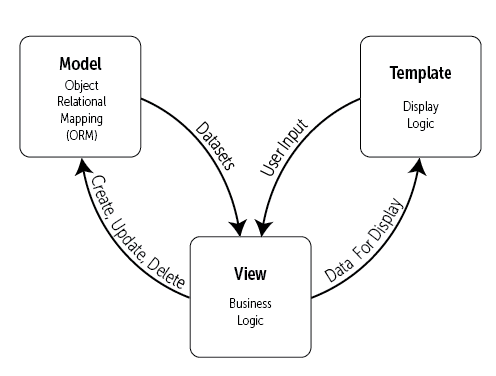
\includegraphics[scale=0.75]{figures/mtv.png}
    \caption{نحوه ارتباط لایه‌های جنگو}
    \label{mtv}
\end{figure}


\subsubsection{امکان استفاده موثر از سطح بالایی از تجرید و انتزاع}
جنگو در بسیاری از موارد با استفاده از مفهوم انتزاع، سهولت زیادی را فراهم کرده است. برای مثال برای کار با تکنولوژی‌هایی چون پروتکل انتقال پرونده\LTRfootnote{\lr{File Transfer Protocol;{FTP}}} یا زبان نشانه‌گذاری ابرمتنی\LTRfootnote{\lr{HyperText Markup Language}}، با یک مفهوم انتزاعی و سطح بالا روبرو خواهیم بود که با استفاده از روابط و توابع متعدد، برنامه‌نویسی را بسیار آسان و قدرتمند می‌کند.
 
علاوه بر موارد ذکر شده، جنگو ویژگی‌های دیگری نیز دارد. از جمله:
\begin{itemize}
	\item امکان تعیین اینکه کدام کد یا توابع مسئول جواب دادن به آدرس درخواست داده شده هستند.
	\item تسهیل نمایش، اعتبارسنجی و نمایش فرم‌های ساخته شده از زبان نشانه‌گذاری ابرمتنی یکی از مهترین روش‌ها برای دریافت اطلاعات از یک کاربر وب است.
	\item حذف پسوند فایل از آدرس‌‌های وب (مثلا \lr{aspx.} یا \lr{php.})
\end{itemize}
 
\subsection{تاثیر پایتون بر روی جنگو}
همانطور که اشاره شد، جنگو بر اساس زبان برنامه‌نویسی پایتون نوشته شده که باعث شده است تا ویژگی‌های زبان پایتون برای جنگو نیز به ارث رسیده باشد. در زیر به برخی از این ویژگی‌ها اشاره شده است:
\begin{itemize}
	\item پایتون زبانی تفسیری\LTRfootnote{\lr{interpretive}} بوده و برای اجرا نیازی به کامپایل ندارد. این ویژگی باعث می‌شود که بعد از تغییر کد، نتایج کار بلافاصله قابل مشاهده باشد.
	\item داده‌ها و متغیر‌ها در پایتون پویا و بدون نیاز به تعریف نوع\LTRfootnote{\lr{Type}} هستند.
	\item نحو زبان پایتون کوتاه و در عین حال واضح و قابل فهم است. این ویژگی باعث می‌شود که برای انجام کارهای مشابه در زبان‌های برنامه‌نویسی دیگر، به نسبت کدنویسی کمتری انجام شود.
\end{itemize}

 
\subsection{بخش‌های جنگو}
در هسته جنگو، برای راحتی و سهولت کار بخش‌هایی طراحی و پیاده‌سازی شده است. برخی از 
این بخش‌ها عبارتند از:
\begin{itemize}
	\item میزبان وب مستقل و کوچک برای آزمون\LTRfootnote{\lr{Test}} برنامه 
	\item سیستمی برای معتبرسازی\LTRfootnote{\lr{Validation}} و سری‌سازی\LTRfootnote{\lr{Serialization}} فرم‌هایی با  زبان نشانه‌گذاری ابرمتنی
	\item چهارچوبی برای نهان‌سازی اطلاعات جهت استفاده مجدد با استفاده از حافظه نهان\LTRfootnote{\lr{Cache}} که روش‌های مختلف ذخیره و بازیابی حافظه نهان را در اختیار قرار می‌دهد .
	\item پشتیبانی از ابزارهای میانی\LTRfootnote{\lr{Middleware}} که امکان اجرای توابع و دستورات مورد نظر را در مراحل مختلف پردازش یک درخواست ،فراهم می‌کند.
	\item یک توزیع‌کننده\LTRfootnote{\lr{Dispatcher}} درونی که به بخش‌های مختلف برنامه امکان دریافت سیگنال‌ها و رویدادهای مختلف را می‌دهد.
	\item سیستم بین‌الملل‌سازی\LTRfootnote{\lr{Internationalization}} که حتی امکان ترجمه بخش‌های مختلف جنگو به زبان‌های مختلف را فراهم می‌کند. از این ویژگی جهت تنظیم ساعت محلی نیز استفاده می‌شود.
	\item  سیستمی برای تسلسل و سری‌سازی که امکان کار با انواع داده‌های مبتنی بر زبان نشانه گذاری امتدادپذیر\LTRfootnote{\lr{eXtensible Markup Language (XML)}} و نماد شئ جاوااسکریپت\LTRfootnote{\lr{JavaScript Object Notation (JSON)}} را فراهم می کند .
	\item سیستمی برای توسعه قابلیت‌های موتور قالب. مانند تعیین دسترسی برای هر بخش مختلف از سایت.
\end{itemize}
 
همچنین بسته جنگو شامل ابزارها و برنامه‌های جانبی مختلفی است که در داخل بسته \lr{contrib} قرار دارند. برخی از این ابزار ها عبارتند از:
\begin{itemize}
	\item سیستم تصدیق و شناسایی کاربر\LTRfootnote{\lr{Authentication}}
	\item سیستم تعیین دسترسی به کاربر\LTRfootnote{\lr{Authorization}}
	\item رابط مدیریتی پویا
	\item ابزارهایی برای ایجاد \lr{RSS} و \lr{Atom}
	\item سیستم نظر‌دهی انعطاف‌پذیر
	\item یک چارچوب برای ایجاد برنامه‌های کاربردی \lr{GIS}
	\item ابزارهایی برای تولید نقشه سایت\LTRfootnote{\lr{Sitemap}}
	\item ابزارهای امنیتی برای جلوگیری از حملات \lr{CSRF}
	\item کتابخانه‌های قالب که امکان استفاده از زبان‌های نشانه‌گذاری کم حجم مانند \lr{Textile} و \lr{Markdown} را فراهم می‌سازد.
\end{itemize}
 
\subsection{انطباق با میزبان‌های مختلف}
جنگو با استفاده از واحد\LTRfootnote{\lr{Module}} \lr{mod\_python} به‌خوبی بر روی میزبان‌های وب آپاچی\LTRfootnote{\lr{Apache}} قابل اجرا است. همچنین بر روی تمامی میزبان‌هایی که از \lr{WSGI}پشتیبانی می‌کنند قابل اجرا است. به غیر از موارد ذکر شده، جنگو توانایی راه‌اندازی سرور \lr{FastCGI} را دارا است.
 
\section{چهارچوب نرم‌افزاری \lr{REST} جنگو}
برای آشنایی با این چهارچوب، ابتدا دو موضوع رابط‌برنامه‌نویسی نرم‌افزار\LTRfootnote{\lr{Application Programming Interface (API)}} و \lr{REST} باید توضیح داده شود.
 
\subsection{رابط برنامه‌نویسی نرم‌افزار چیست؟}
در حوزه توسعه نرم‌افزار، واژه‌ رابط برنامه‌نویسی نرم‌افزار بسیار تکرار می‌شود. در واقع، از آنجا که می‌توان واژه \lr{Interface} را به «فصل مشترک» در فارسی ترجمه کرد، می‌توان گفت که رابط برنامه‌نویسی نرم‌افزار فصل مشترکی مابین دو نرم‌افزار یا اپلیکیشن است.
\subsubsection{آشنایی با انواع رابط‌های برنامه‌نویسی نرم‌افزار}
با در نظر گرفتن این نکته که رابط‌ برنامه‌نویسی نرم‌افزار سازوکاری است که از طریق آن تعامل سیستم با سیستم به جای تعامل کاربر با سیستم صورت می‌گیرد، می‌توان دسته‌بند‌ی‌های مختلفی در نظر گرفت که عبارتند از:

\begin{itemize}
	\item رابط برنامه‌نویسی در سخت‌افزار
	\item رابط برنامه‌نویسی نرم‌افزاری در سطح سیستم‌عامل
	\item رابط برنامه‌نویسی نرم‌افزاری در زبان‌های برنامه‌نویسی
	\item کیت‌های توسعه نرم‌افزار\LTRfootnote{\lr{Software Development Kit (SDK)}}
	\item رابط برنامه‌نویسی نرم‌افزاری تحت وب (وب سرویس)
\end{itemize}
 

\subsubsection{تقسیم‌بندی رابط‌های برنامه‌نویسی نرم‌افزار از بُعد سطح دسترسی}
علاوه بر تقسیم‌بندی‌های فوق،‌ رابط برنامه‌نویسی نرم‌افزارهای تحت وب را می‌توان از نقطه نظر سطح دسترسی به دسته‌های مختلفی تقسیم‌بندی کرد که عبارتند از:
\begin{itemize}
	\item رابط برنامه‌نویسی نرم‌افزار باز\LTRfootnote{\lr{Open API}}: این دست رابط‌های برنامه‌نویسی نرم‌افزار که اصطلاحاً \lr{Public APIs} نیز نامیده می‌شوند، بدون هیچ‌گونه محدودیت در سطح دسترسی برای کاربردهای مجموعه‌های تجاری به مشتری\LTRfootnote{\lr{Business to Customer (B2C)}}، در اختیار برنامه‌نویس‌ها قرار می‌گیرند.
	\item رابط برنامه‌نویسی نرم‌افزار شریک\LTRfootnote{\lr{Partner API}}: این گروه از رابط‌های برنامه‌نویسی نرم‌افزار صرفاً در اختیار کسب‌وکارهای به اصطلاح تجاری به تجاری\LTRfootnote{\lr{Business to Business (B2B)}} و تجاری به مشتری است و برخلاف مورد قبل هر برنامه‌نویسی به آن‌ها دسترسی ندارد؛ برای استفاده از آن‌ها معمولا باید هزینه کرد.
	\item رابط برنامه‌نویسی نرم‌افزار داخلی \LTRfootnote{\lr{Internal API}}: این گروه از رابط‌های برنامه‌نویسی نرم‌افزار که تحت عنوان \lr{Private APIs} نیز شناخته می‌شوند، صرفاً برای استفاده‌های داخلی یک سیستم طراحی می‌شوند.

\end{itemize}

\subsection{\lr{REST} چیست؟}
با توجه به تعریف
\lr{REST}\LTRfootnote{\lr{Representational State Transfer}} يك مدل معماري براي طراحي برنامه‌هاي كاربردی شبكه است. ايده اصلي این معماری اين است كه به جاي استفاده از مكانيزم‌هاي پيچيده‌اي مانند \lr{CORBA}، \lr{RPC} يا \lr{SOAP} براي اتصال ماشين‌ها، از \lr{HTTP} و به سادگی براي برقراري ارتباط بين ماشين‌ها استفاده شود.\\
این مدل دارای ویژگی‌های زیر است: 
\begin{itemize}
	\item بر پایه مشتری-میزبان\LTRfootnote{\lr{client-server}} است.
	\item بدون حالت\LTRfootnote{\lr{Stateless}} است.
	\item از حافظه نهان\LTRfootnote{\lr{Cache}} پشتیبانی می‌کند.
	\item سيستم لايه‌بندي شده است.
    \item دارای واسط واحد\LTRfootnote{\lr{Uniform Interface}} است.
\end{itemize}
 
به سيستمي كه اين قيود را رعايت نمايد، \lr{RESTful} مي‌گويند. از لحاظ رويكرد برنامه‌نويسي \lr{REST} جايگزيني ساده براي سرويس‌هاي وب است. توسعه‌پذيري در تعاملات ميان اجزا، عموميت واسط‌ها و توسعه مستقل اجزا از كليدي‌ترين اهداف این معماری است.

استفاده از معماري \lr{REST} در برنامه‌نويسي، كارايي، سادگي، انعطاف‌پذيري، امكان مشاهده و نظارت، قابليت حمل و قابليت اطمينان را افزايش مي دهد.
امروزه برنامه‌های سنتی وب در حال حرکت به سمت سرویسی شدن هستند. بدین صورت که برنامه سمت مشتری تنها از طریق وب‌سرویس‌ها با سرور در تماس هستند. به بیانی دیگر ارتباط سمت مشتری با لایه داده برنامه، از طریق وب‌سرویس‌ها صورت می‌پذیرد. در چنین برنامه‌هایی منطق برنامه کاملا در سمت مشتری پیاده‌سازی می‌شود و سمت میزبان دیگر هیچ نقشی جز فراهم‌کردن داده برای برنامه‌های سمت مشتری را برعهده ندارد.
 
یکی از نکات مثبت این معماری این است که دسترسی برنامه سمت مشتری به منابع، از طریق درخواست‌های \lr{HTTP} انجام می‌گیرد. این درخواست‌ها با روش\LTRfootnote{\lr{Method}}های مختلفی می‌توانند ارسال شوند که هر یک معنا و مفهومی خاصی دارد. هریک از این روش‌ها در زیر تعریف شده‌اند:
\begin{itemize}
	\item روش \lr{GET} به‌منظور بازیابی و خواندن منبع استفاده می شود.
	\item روش \lr{POST} زمانی استفاده می‌شود که بخواهیم منبع جدیدی را ایجاد کنیم.
	\item روش \lr{DELETE} به‌منظور حذف یک منبع مورد استفاده قرار می‌گیرد.
	\item روش‌های \lr{PUT} و \lr{PATCH} برای دست‌کاری در یک منبع مورد استفاده قرار می‌گیرند.
\end{itemize}


\subsection{جنگو \lr{REST}}
چهارچوب نرم‌افزاری جنگو \lr{REST}\cite{DjangoREST}، یک ابزار قدرتمند و انعطاف‌پذیر برای ساختن رابط‌های برنامه‌نویسی نرم‌افزارهای شبکه وب است.
برخی از ویژگی‌های این چهارچوب نرم‌افزاری به صورت زیر است:
\begin{itemize}
	\item خط مشی‌های تأیید اعتبار شامل بسته‌هایی برای \lr{OAuth1a} و \lr{OAuth2}
	\item پشتیبانی از منابع داده \lr{ORM}\LTRfootnote{\lr{Object-Relational Mapping}} و غیر \lr{ORM}
	\item مستندات گسترده و پشتیبانی 
	\item مورد استفاده و مورد اعتماد شرکت‌های معتبر بین المللی از جمله موزیلا، \lr{Red Hat}، \lr{Heroku} و \lr{Eventbrite} است.
\end{itemize}


\section{چهارچوب نرم‌افزاری \lr{Vue.js}}
\lr{Vue.js}\cite{Vue} یک چارچوب متن باز \lr{JavaScript} برای ساخت رابط‌های کاربری\LTRfootnote{\lr{User Interface}} و برنامه‌های تک‌صفحه‌ای\LTRfootnote{\lr{Single Page Application}} است. این چهارچوب نخستین بار توسط ایوان یو\LTRfootnote{\lr{Evan You}} ایجاد شده است و اکنون توسط او و بقیه اعضای تیم اصلی که از شرکت‌های مختلفی چون \lr{Netlify} و \lr{Netguru} آمده‌اند، نگهداری می‌شود.

در ادامه برخی از ویژگی‌های این چهارچوب توضیح داده خواهد شد.

\subsection{اجزاء}
هدف این اجزا\LTRfootnote{\lr{Componenets}}، افزایش استفاده مجدد از کد است. در مواقعی که در چندین بخش مختلف به یک المان خاص در طراحی صفحات نیاز است، از این اجزا استفاده می‌شود.

\subsection{قالب‌ها}
\lr{Vue} از یک نحو\LTRfootnote{\lr{Syntax}} که مشابه قوانین نوشتاری زبان نشانه‌گذاری ابرمتنی است، استفاده می‌کند. همه قالب‌های \lr{Vue} دارای زبان نشانه‌گذاری ابرمتنی معتبری هستند که توسط مرورگرهای استاندارد قابل تجزیه\LTRfootnote{\lr{Parse}} است. \lr{Vue} این امکان را می‌دهد تا قالب‌ها قبل از بروزرسانی مرورگر، تغییرات لازم را اعمال کنند.

کاربران \lr{Vue} می توانند از نحو استاندارد در قالب‌ها استفاده کنند و مستقیماً و با استفاده از \lr{JSX} بنویسند.


\subsection{انتقال‌ها}
{\lr{Vue}} روش‌های مختلفی را برای اعمال جلوه‌های انتقال \LTRfootnote{\lr{Transitions}}هنگام وارد کردن، به روزرسانی یا حذف شدن از \LTRfootnote{\lr{Document Object Model}}\lr{DOM} را فراهم کرده است. این موارد عبارتند از:

\begin{itemize}
   	\item اعمال خودکار کلاس‌ها برای انتقال‌ها و انیمیشن‌های \lr{CSS}
   	\item تعامل با کتابخانه‌های شخص ثالث \lr{CSS}، مانند \lr{Animate.css}
   	\item تعامل با کتابخانه‌های شخص ثالث جاوا اسکریپت ، مانند \lr{Velocity.js}
\end{itemize}




\subsection{چهارچوب نرم‌افزاری \lr{Nuxt.js}}
\lr{Nuxt.js}\cite{Nuxt} یک چارچوب برنامه وبِ منبع آزاد و مبتنی بر \lr{Vue.js} ، \lr{Node.js} ، \lr{Webpack} و \lr{Babel.js} است.
  ابتدا به معرفی \lr{Vue.js} پرداخته می‌شود.

از مزایای استفاده از این چهارچوب\LTRfootnote{\lr{Framework}}، کاهش زمان پاسخگویی برنامه و همچنین بهبود بهینه سازی موتور جستجو\LTRfootnote{\lr{SEO}} در مقایسه با سایر برنامه‌های تک‌صفحه‌ای است. دلیل کاهش زمان تعامل این است که محتوای کامل هر صفحه، قبل از اجرای جاوا اسکریپت در برنامه سمت مشتری، توسط وب سرور ارائه\LTRfootnote{\lr{Render}} می‌شود. به بیان دیگر، با استفاده از این چهارچوب، به‌طور همزمان از مزایای نمایش سنتی \lr{HTML} و همچنین نمایش به وسیله برنامه‌های تک‌صفحه‌ای جدید بهره برده می‌شود.
اما فایده اصلی این چهارچوب، ساده‌سازی و یکپارچه‌سازی پروژه سمت کاربر برای برنامه‌نویس است.


\section{پایگاه‌داده رابطه‌ای \lr{Postgress}}
\lr{Postgress}\cite{Postgress}، که همچنین با عنوان \lr{Postgres} شناخته می‌شود، یک سیستم مدیریت پایگاه‌داده رابطه‌ای\LTRfootnote{\lr{Relational}} آزاد و متن‌باز است. ابتدا به مفاهیم پایگاه‌داده رابطه‌ای پرداخته می‌شود و سپس پایگاه‌داده \lr{Postgress} معرفی می‌گردد.
 
\subsection{پایگاه داده رابطه‌ای}
پایگاه داده رابطه‌ای به آن دسته از پایگاه‌های داده اطلاق می‌شود که بر اساس مدل رابطه‌ای طراحی و ایجاد شده باشند. پس از پایگاه‌های داده‌ای سلسله مراتبی و شبکه‌ای، که هر یک دارای ضعف‌هایی بودند، متخصصان در جستجوی مدلی بودند که دارای ساختار داده‌ای با انتزاع قوی باشد. مدل رابطه‌ای در سال ۱۹۷۰ توسط ادگار کاد\LTRfootnote{\lr{Edgar F.Codd}} مطرح شد. این مدل دارای ساختار داده‌ای با انتزاع قوی بوده و اساساً ساختار داده‌ای در آن بر اساس یک مفهوم ریاضی به نام رابطه استوار است. در اینجا لازم است به این نکته توجه شود که مفهوم رابطه با مفهوم ریاضی آن تاحدودی متفاوت است.
 
برای طراحی پایگاه داده‌ها در سطح انتزاعی پایین‌تر از سطح مدل‌سازی، به یک ساختار داده‌ای از یک مدل داده‌ای نیاز است و اساساً همین مدل داده‌ای تأمین‌کننده محیط انتزاعی است. در پایگاه داده رابطه‌ای بالاخص در محیط انتزاعی مورد استفاده کاربر، رابطه نمایشی جدولی دارد و اساساً پایگاه داده رابطه‌ای مجموعه‌ای است از تعدادی نوع جدول. مفاهیم ساختار جدولی عبارتند از: سطر، جدول و ستون
هر جدول از نظر محتوای داده‌ای مجموعه‌ای است از نمونه‌های متمایز از انواع سطرها و هر سطر نیز مجموعه‌ای از مقادیر است که هر کدام از یک مجموعه برگرفته شده‌اند. به هر یک از عناصر سطر یک ستون گویند. لازم است ذکر شود که در ساختار جدولی، تنها عنصر ساختاری اساسی همین مفهوم نوع جدول است.
 
\subsubsection{ویژگی‌های رابطه}
رابطه به عنوان تنها عنصر ساختاری اصلی در مدل رابطه‌ای برای نمایش انواع موجودیت‌ها و انواع ارتباطات به کار می‌رود. در واقع در مدل رابطه‌ای هم نوع موجودیت و هم نوع ارتباط با مفهوم رابطه نمایش داده می‌شوند و در نتیجه هم نمونه موجودیت و هم نمونه ارتباط با مفهوم تاپل نشان داده می‌شوند. رابطه دارای چهار ویژگی زیر است:
\begin{itemize}
  	\item رابطه تاپل تکراری ندارد، زیرا بدنه رابطه مجموعه‌است و مجموعه نمی‌تواند عنصر تکراری داشته باشد.
	\item تاپل‌ها نظم ندارند زیرا بدنه رابطه مجموعه‌ است و مجموعه در حالت کلی فاقد نظم است.
	\item صفات رابطه نظم مکانی ندارند زیرا سرآیند، رابطه مجموعه‌است و مجموعه در حالت کلی فاقد نظم است.
	\item تمام صفات تک مقداری (تجزیه نشدنی) هستند زیرا در نمایش جدولی رابطه، در تقاطع هر سطر و ستون باید یک مقدار وجود داشته باشد.
\end{itemize}

 
\subsubsection{انواع کلیدها در مدل رابطه‌ای}

\begin{itemize}
  	\item ابر کلید: هر ترکیبی از صفات جدول را که یکتایی مقدار داشته باشد، ابر کلید گویند. به بیانی دیگر هر زیر مجموعه عنوان رابطه را دارد، که یکتایی مقدار در بدنه رابطه را داشته باشد. تعریف دیگر ابر کلید عبارت است از هر ترکیبی از اسامی صفات رابطه که در هیچ دو تاپل مقدار یکسان نداشته باشد.

  	\item کلید کاندید: کلید کاندید امکانی است برای ارجاع به «تک تاپل» در رابطه. مجموعه صفات \lr{k} از رابطه\lr{R} یک کلید کاندید است، اگر دارای خاصیت غیر کاهشی و یکتایی باشد.

  	\item کلید اصلی: 
  	\item یکی از کلیدهای کاندید رابطه که شرایط زیر را داشته باشد:
	\begin{enumerate}
		\item شناسایی‌کننده نوع موجودیت در رابطه باشد. مانند شماره عضویت کتابخانه برای هر دانشجو.
		\item از نظر طول، کوتاه‌تر باشد. یعنی بین دو کلید کاندید، کلید کوتاه‌تر برای کلید اصلی بودن بهتر است.
	\end{enumerate}
  	\item کلید جانشین: هر کلید کاندید به غیر از کلید اصلی را کلید جانشین گویند.
  	\item کلید خارجی: دو رابطه \lr{R1} و \lr{R2} را در نظر بگیرید. هر زیر مجموعه از صفات رابطه \lr{R2}که هر مقدار معلوم آن با یک مقدار از کلید کاندید \lr{R1}برابر باشد، کلید خارجی در رابطه \lr{R2}است. نقش کلید خارجی برای نمایش ارتباطات بین انواع موجودیت‌ها و در نتیجه بین نمونه‌های آنها به کار می‌رود.

\end{itemize}


 
\subsection{پایگاه‌داده \lr{Postgress}}
\lr{Postgress} یک سامانه مدیریت پایگاه داده‌های رابطه‌ای است که برای سیستم‌های مختلفی از جمله لینوکس، فری بی‌اس‌دی\LTRfootnote{\lr{FreeBSD }}، ویندوز و مک اواس\lr{macOS} موجود است. این پایگاه‌داده توسط گروه توسعه سراسری \lr{Postgresql} توسعه داده می‌شود، که شامل تعداد زیادی از افراد داوطلب است. این پایگاه‌داده بر توسعه‌پذیری و رعایت استانداردهای فنی تأکید دارد. همچنین توانایی پاسخگویی به بار کاری زیاد، در مقیاس یک کامپیوتر تا انبارهای داده،\LTRfootnote{\lr{Data Warehouse}} برای استفاده همزمان کاربران را دارد.
 
تراکنش‌های \lr{PostgreSQL} شامل ویژگی‌های زیر است:
\begin{itemize}
  	\item اتمی\LTRfootnote{\lr{Atomicity}}
	\item پایداری\LTRfootnote{\lr{Consistency}}
	\item ایزوله\LTRfootnote{\lr{Isolation}}
	\item با دوام\LTRfootnote{\lr{Durability}}
	\item بروزرسانی خودکار نمایه‌ها\LTRfootnote{\lr{Automatically Updatable Views}}
	\item پشتیبانی از تریگر\LTRfootnote{\lr{Trigger}}
	\item پشتیبانی از کلید‌های خارجی
	\item پشتیبانی از توابع تجمیعی
	\item کلید‌های خارجی
	\item پشتیبانی از رویه‌های ذخیره‌شده\LTRfootnote{\lr{Stored Procedures}}
\end{itemize}


\section{ماشین مجازی}
برای پیاده‌سازی این پروژه در محیط عملیاتی از میزبان مجازی شخصی\LTRfootnote{\lr{Virtual Private Server (VPS)}} استفاده شده است. برای این که بدانیم میزبان مجازی شخصی چیست، ابتدا باید با ماشین مجازی\LTRfootnote{\lr{Virtual Machine}} آشنا شویم. یک ماشین مجازی از منابع فیزیکی یک کامپیوتر استفاده می کند. این منابع می توانند پردازنده، حافظه رم و یا دیسک‌های ذخیره‌سازی باشند. ماشین‌های مجازی با بهره‌گیری از این منابع، یک نوع از کامپیوتر را شبیه‌سازی می‌کنند.
برای درک بهتر، کافی است امکان تصویر در تصویر یک تلویزیون را تصور کنید. یک تلویزیون امروزی می‌تواند همزمان دو تصویر از دو شبکه متفاوت را پخش کند. این امکان در حالی برای شما فراهم می‌شود که در حال استفاده از یک تلویزیون هستید؛ اما نتیجه‌ای که حاصل می‌شود، دو تصویر همزمان است. پس در این حالت از یک منبع واحد، حداقل دو خروجی دریافت کرده‌اید. پس یک یا چند ماشین‌ مجازی می‌تواند درون یک سخت‌افزار یک کامپیوتر واحد اجرا شود. به‌عنوان مثال می‌توان یک ماشین‌ مجازی با سیستم‌عامل ویندوز را درون یک کامپیوتر که خود نیز از سیستم‌عامل ویندوز بهره می‌برد اجرا کرد.
این امکان وجود دارد که چندین سیستم‌عامل را از طریق ماشین‌های مجازی به واسطه یک سخت‌افزار واحد اجرا کرد. این دقیقا همان کاری است که شرکت های ارائه میزبانی\LTRfootnote{\lr{Hosting}} انجام می‌دهند. اما این بار تفاوت آن‌جا است که آن‌ها به جای کامپیوترهای شخصی از سرورهای پرقدرت استفاده می‌کنند. سرورهایی که هرکدامشان می‌توانند بیش از 48 هسته پردازشگر و بیش از 1 ترابایت حافظه رم داشته باشند. تعداد زیادی از این سرورها در محل‌هایی به نام مراکز داده\LTRfootnote{\lr{Data center}} نگه‌داری می شوند. هر مرکز داده نیز می‌تواند بیش از صدها و شاید هزاران سرور را درون خود جای دهد. هر کدام از این سرورها نیز توانایی اجرای چندین و شاید صدها ماشین مجازی را دارند.
این ماشین‌های مجازی می‌توانند توسط سازمان‌ها، ادارات و یا حتی افراد استفاده شوند. اگر یک ماشین مجازی اجاره داده شود، اصطلاحا به آن سرور اختصاصی مجازی یا میزبان مجازی شخصی می‌گویند. پس بنابراین یک میزبان مجازی شخصی یک ماشین مجازی به حساب می‌آید و فقط نام تجاری به خود گرفته‌است.
 
\subsection{دلایل استفاده از میزبان مجازی شخصی}
میزبان مجازی شخصی به عنوان یک سرویس به کاربر ارائه می‌شود. اما دیگر سرویس‌هایی که در مقابل میزبان مجازی شخصی قرار می‌گیرند، هاست‌های اختصاصی و هاست‌های اشتراکی هستند.
هاست‌های اختصاصی به صورت کامل در اختیار کاربران قرار می‌گیرند. به این صورت که مشتری یک سرور کامل را اجاره کرده و آن را در تحت نظارت و استفاده می‌گیرد. به این ترتیب هیچ‌کس دیگری به آن سخت‌افزار دسترسی نداشته و کنترل کامل سخت افزار در اختیار اجاره کننده‌است.
درمقابل، هاستینگ اشتراکی بدین معناست که در یک سرور واحد، چندین برنامه اجرا شده و چندین مشتری همزمان از سخت‌افزار استفاده می‌کنند.
هاست‌های اختصاصی معمولا از منابع سخت‌افزاری غنی‌تری نسبت به میزبان مجازی شخصی بهره برده و البته اجاره آن‌ها نیز بسیار گران است. درحالی که اجاره میزبان‌های اشتراکی نسبت به هاست‌های اختصاصی ارزان‌تر بوده ولی به هیچ عنوان انعطاف‌پذیری میزبان مجازی شخصی را ندارند.
می‌توان گفت اجاره یک میزبان مجازی شخصی نیز فقط کمی گران‌تر از هاست‌های اشتراکی است. 
میزبان مجازی شخصی قابل انعطاف است. چرا که شما تقریبا هرکاری را می‌توانید با یک ماشین مجازی ویندوزی انجام دهید. می توان از یک میزبان مجازی شخصی به‌عنوان فضایی برای ذخیره‌سازی اطلاعات شخصی استفاده کرد.

نکته ای راجع به یک میزبان مجازی شخصی باید در نظر گرفته شود، این است که درصورت استفاده نادرست از آن، کاربر نمی‌تواند هیچ‌گونه آسیبی به سرور اصلی بزند. به عنوان مثال اگر یک میزبان مجازی شخصی آلوده به ویروس شود، دیگر ماشین‌های مجازی موجود در سرور در امان خواهند بود و کوچک‌ترین اختلالی در نحوه سرویس‌دهی آن‌ها پیش نخواهد آمد.
یک میزبان مجازی شخصی می‌تواند به راحتی راه‌اندازی مجدد شده و یا حتی در عرض چند دقیقه دوباره با یک سیستم‌عامل جدید در اختیار کاربر قرار گیرد. تنها نکته‌ای که باید مدنظر داشت، تهیه نسخه پشتیبان از اطلاعات حیاتی است، چرا که آن ها هنگام نصبِ دوباره سیستم‌عامل از بین خواهند رفت.
ماشین‌های مجازی ایمن هستند. به این معنی که هر ماشین مجازی به صورت جداگانه از منابع استفاده کرده و دسترسی کاربران به ماشین مجازی فرد دیگری، غیرممکن است.
اما این مهم درصورت استفاده از میزبان‌های اشتراکی کمی متفاوت است. به دلیل قرارگیری اپلیکیشن‌ها و یا وب‌سایت ها در کنار همدیگر و مدیریت آن‌ها توسط نرم‌افزاری واحد مانند وب‌سرورها؛ امکان این که دیگر اپلیکیشن ها مورد سوءاستفاده توسط دیگر کاربران قرار گیرد، وجود دارد.
 

\subsection{موارد استفاده از میزبان مجازی شخصی}
در ذیل به مواردی خواهیم پرداخت که با استفاده از یک میزبان مجازی شخصی می توان به آن‌ها دست پیدا کرد.

\subsubsection{اجرای یک وب‌سایت}
این روزها بهترین راه اجرای یک وب‌سایت از طریق میزبان مجازی شخصی است. معمولا برای یک میزبان مجازی شخصی منابع اختصاصی در نظر گرفته می‌شود. به این‌صورت که بخشی از منابع که اختیار کرده اید، همواره در اختیار شما خواهد بود و برنامه دیگری امکان اشغال آن را ندارد.

\subsubsection{ایجاد یک سرور یا سرویس}
شاید یک سازمان، شرکت و یا حتی اشخاص بخواهند برای خود سرویس ایمیل اختصاصی داشته باشند. با استفاده از میزبان مجازی شخصی و نرم‌افزار سرویس ایمیل می‌توان سرور اختصاصی پست الکترونیک خود را داشته و شخصا آن را مدیریت کرد. این راه کار بسیار مورد استقبال شرکت‌ها قرار گرفته است.


\subsubsection{ایجاد یک محیط آزمایشی}
با استفاده از یک میزبان مجازی شخصی می‌توان به آزمایش و اصلاح انواع نرم افزارهای گوناگون پرداخت. اشاره شد که اگر اتفاق ناگواری برای یک میزبان مجازی شخصی بیافتد دیگر ماشین‌های مجازی از این رخداد صدمه‌ای نخواهند دید. درصورتی که سیستم‌عامل یک میزبان مجازی شخصی دچار اشکال شود، به راحتی هرچه تمام‌تر می توان سیستم‌عامل جدیدی را جایگزین کرد. این در صورتی است که اگر این اتفاق برای یک هاست اختصاصی رخ دهد، نصب و راه‌اندازی یک سیستم‌عامل جدید کاری پردردسر و زمان‌بر خواهد بود.


\section{نتیجه‌گیری}
همانطور که در قسمت‌های مختلف این بخش به تفصیل توضیح داده شد، این پروژه از قطعات سخت‌افزاری، تکنولوژی‌های نرم‌افزاری و همچنین محیط‌هایی برای عملیاتی کردن استفاده شده است. برای پیاده‌سازی سخت‌افزاری پروژه از بورد رزبری‌پای مدل \lr{3A} استفاده شد. همچنین جهت تعامل این بورد با کاربر، از نمایشگر لمسی \lr{3.5} اینچی \lr{Waveshare} استفاده شد. برنامه‌ای که بر روی نمایشگر نمایش داده می‌شود، با استفاده از چهارچوب نرم‌افزاری سمت کاربر \lr{Nuxt.js} که خود بر پایه \lr{Vue.js} نوشته شده است، برنامه‌نویسی شد. این برنامه با استفاده از وب‌سرویس \lr{REST} با چهارچوب نرم‌افزاری \lr{Django} در تعامل است.

برای عملیاتی کردن پروژه بر روی محیطی که همه کاربران به برنامه‌ها دسترسی داشته باشند از ماشین مجازی استفاده شد.



